\documentclass[english,11pt,a4paper]{article}
\usepackage{fontspec}
\setmainfont{Times New Roman}
\usepackage{pdflscape}
\usepackage[figuresright]{rotating}
\usepackage{appendix}

\usepackage[a4paper,top=2cm,bottom=2cm,left=2cm,right=2cm,marginparwidth=1.75cm]{geometry}
\usepackage[affil-it]{authblk}
\usepackage{float}

\usepackage[style=apa,natbib=true,backend=biber]{biblatex}
\addbibresource{ref.bib}

\usepackage[colorlinks=true, allcolors=blue]{hyperref}

% for typesetting mathematical formulas and symbols.
\usepackage{amsmath}
\usepackage{mathdots}
\usepackage{yhmath}
\usepackage{amssymb}

\usepackage{epigraph}
\usepackage{graphicx}

% extra formatting commands for tables
\usepackage{booktabs}
\usepackage{array}
\usepackage{threeparttablex}
\usepackage{tabularray}
\usepackage{dcolumn}
\usepackage{tablefootnote}
\usepackage{longtable}

\usepackage{url}
\urlstyle{same}

\usepackage{amsthm}
\usepackage{nameref}
\theoremstyle{definition}
\newtheorem{question}{Question}
\newtheorem{assumption}{Assumption}
\newtheorem*{premise*}{Premise}
\newtheorem*{conclusion*}{Conclusion}

\makeatletter
\patchcmd{\thmhead}{(#3)}{\textbf{ #3}}{}{}
\makeatother

\usepackage{etoolbox}
\makeatletter
\pretocmd{\appendices}{
	\let\addcontentsline\@gobblethree
	\renewcommand{\thesection}{Appendix \arabic{section}}
}{}{}
\makeatother

\begin{document}

\title{Equality of Opportunity or Meritocracy: Is it Fair?}
\author{}
\date{}
\maketitle

\begin{abstract}
	\noindent
	This research explores the paradoxes of meritocracy using two distinct investigations. The first, employing Boolean analysis, uncovers an irony in meritocracy: it is perceived as fair, yet it downplays hard work (the very architect of fairness) and favors talent. It proposes three potential conditions (not necessarily simultaneously) for a logical meritocracy: difference legitimation, absence of genetic constraints on capabilities, or the use of effort as the yardstick for merit. The second investigation, utilizing Machine Learning on data from the European Social Survey round 9, underscores that meritocratic equality of opportunities goes hand in hand with the belief in social privilege. This bolsters the viewpoint that belief in meritocracy is associated with social inequality. The research concludes by endorsing the development of a novel form of meritocracy.
\end{abstract}

\vspace{1em}
\noindent\textbf{Keywords:} meritocracy, Boolean analysis, Machine Learning, fairness

\vspace{0.5em}
\noindent\textbf{JEL Codes:} D63, I24, Z13
	
\section{Is Meritocracy Just?}
"It's your talent and hard work that matter, not where you were born, who your parents are, or what your accent sounds like," said former British Prime Minister Theresa May on September 9, 2016. She emphasized that her government's priorities were aligned with those of ordinary, working-class people and that their actions would be driven by the interests of the many, not the privileged few. Similarly, in the US, \citet{ries2011lean}, the author of "The Lean Startup" and an advocate for lean startup principles, stated that "Meritocracy is a good thing. Whenever possible, people should be judged based on their work and results, not superficial features." Meritocracy represents a source of justice for the working class and provides hope for social mobility in a world where injustices based on gender \citep{belingheri2021twenty} or race \citep{becares2015understanding} still exist. However, as \citet{hayes2013twilight}, the author of the book "Twilight of the Elites: America After Meritocracy," argues, while meritocracy may seem like an appealing vision, it contains the seeds of its own destruction by conceding inequality, evidenced by Jonathan \citet{mijs2021paradox} who argued that income inequality and belief in meritocracy go hand in hand. Such a society does not elevate individuals to higher classes but instead creates a new class that \citet{jin2020meritocracy} describe as a different form of distinction and exclusion, as observed in China.

Most people, especially young individuals from the working class, work tirelessly day and night for a chance to change their lives and strive for social justice. However, "a belief in meritocracy is not only false: it"s bad for you" Clifton \citet{mark2020belief} expressed his ideas on Princeton University Press. According to Mark, the belief in meritocracy is false because success is not solely determined by merit but influenced by luck and external factors like genetics and upbringing. Embracing meritocracy can have negative consequences, leading to self-centeredness, less self-criticism, and discrimination. It fosters a sense of entitlement by overlooking luck's role, leading to a lack of empathy towards those facing challenges and superficial judgments against others. Similarly, Michael \citet{sandel2020tyranny}, the author of "The Tyranny of Merit: What's Become of the Common Good?" contends that the rhetoric surrounding meritocracy reinforces the belief that success is solely derived from merit. This perception leads the successful to feel deserving of their achievements, giving rise to what Sandel terms the "tyranny of merit." He argues that this emphasis on meritocracy has resulted in a growing disparity between the successful and the less fortunate. These arguments made Marc \citet{plattner2021tyranny} posed the question "Is meritocracy just?" in the Journal of Democracy in January 2021.

\section{The ongoing debates against the fairness of meritocracy}
\subsection{Luck egalitarianism: Merit is just the result of luck}

Meritocracy is a social ideal that has gained popularity in recent times. It is the belief that rewards of life, such as money, power, jobs, and university admission, should be distributed according to skill and effort. The most common metaphor is the ‘even playing field’ upon which players can rise to the position that fits their merit. Conceptually and morally, meritocracy is presented as the opposite of systems such as hereditary aristocracy, in which one's social position is determined by the lottery of birth \citep{mark2020belief}. However, meritocracy is not without its flaws. The belief that success or failure in the world is determined by merit rather than luck is demonstrably false \citep{mark2020belief}. This is largely because merit itself is, in large part, the result of luck. Talent and the capacity for determined effort depend a great deal on one’s genetic endowments and upbringing, which are no different from the lottery of birth \citep{mark2020belief}. Luck intervenes by granting people merit and again by furnishing circumstances in which merit can translate into success. Therefore, it is fairer to seek to eliminate arbitrary advantages arising from luck while preserving differences in outcomes that arise from individual choices and efforts – a belief held by advocates of Luck Egalitarianism \citep{knight2013luck}.

\subsection{Nature or Nurture: Do Genes Limit the Development of a Person's Abilities?}

The concept of meritocracy is often scrutinized through the prism of the nature versus nurture debate. Supporters of meritocracy typically lean towards the ‘nature’ argument, contending that inherent talents and capacities, which are presumably determined by one’s genetic makeup, predispose individuals to succeed in specific fields \citep{harris2021nature}. This perspective implies that meritocratic success is largely a product of genetic endowment. Conversely, critics of meritocracy often champion the ‘nurture’ standpoint. They posit that an individual’s environment, experiences, and education significantly shape their abilities. They argue that a meritocratic system might not be equitable as it overlooks disparities in access to resources and opportunities that can nurture talent \citep{montag2018nature}. This viewpoint implies that a truly fair system would consider not just a person’s skills, but also the environment in which those skills were nurtured. Nevertheless, it remains ambiguous whether the ‘nurture’ perspective is more equitable, as children from affluent families have more opportunities to hone their abilities compared to those from impoverished backgrounds. The only potentially justifiable aspect of the ‘nurture’ argument is the high regard for the educational efforts of a less privileged child. This matter will be further elucidated in the ensuing discussion on naturalness bias.
		
\subsection{Naturalness bias: favouring innate talent over hard work}

Meritocracy is seen as a fair way to distribute resources, ensuring the most productive individuals benefit the most. However, the fairness of meritocracy is called into question when considering the naturalness bias, which favours innate talent over hard work \citep{tsay2016privileging, tsay2011naturals}. The naturalness bias is a tendency to value and reward inherent abilities over acquired skills or effort. In a meritocratic system influenced by this bias, individuals with innate talents may have an advantage over those who must put forth more effort to reach the same level of competence. For example, \citet{tsay2011naturals} studied how professionals evaluated "naturals" versus "strivers":

\begin{quote}
Musicians learned about two pianists with equal accomplishments but different backgrounds: one a "natural" with innate talent, the other a "striver" with motivation. Despite expecting strivers to excel, musicians favored naturals, perceiving them as more talented, likely to succeed, and employable.
\end{quote}

This can lead to a disproportionate distribution of rewards, favouring those born with specific talents. Furthermore, this bias overlooks the fact that qualities such as effort, persistence, and resilience are equally crucial for success \citep{tsay2011naturals}, rather than merely relying on one’s inherent abilities. Moreover, if success is predominantly determined by one's inherent abilities, it could be argued that it is not entirely fair because not everyone begins from the same starting point, as discussed about luck egalitarianism above.

\section{The paradox of hard work in a meritocracy}

\epigraph{While meritocracy is a beacon of justice, it ironically undervalues hard work, the very architect of fairness, in favour of talent.}{The author}

In order to address the question of whether meritocracy is just, it is necessary to begin by examining the definition of merit (as shown in Figure~\ref{fig:fig1}). This term was first introduced by Michael \citet{young1958rise}, a British sociologist and politician, in his book ‘The Rise of the Meritocracy.’ According to Young, merit is defined as intelligence combined with effort, and individuals possessing merit are identified at a young age and selected for intensive education. There is also a preoccupation with quantification, test scoring, and qualifications. \citet{ballantine2021sociology} assert that the most prevalent conceptualization of meritocracy defines merit in terms of tested competency and ability, often measured through IQ or standardized achievement tests. However, this definition of merit presents two significant issues. Firstly, the notion of intelligence as solely measured by IQ is overly narrow, as success is not determined exclusively by intelligence. Secondly, even when the concept of intelligence is expanded to encompass talents such as abilities, competence, and skills, the use of IQ as a measure remains inadequate. It raises the question of whether it is equitable to evaluate a child’s potential based on their natural or innate talents and subsequently treat them accordingly. \citet{meyer2022talents} contends that talent can develop over time and that natural factors only contribute to mature talents when external factors are also present. This argument originates from the fundamental issue of whether talent is innate or acquired. The majority of scholars concur that talent comprises both innate and acquired components; while some individuals may possess inherent talents, others may develop them through diligence and practice \citep{meyers2013talent}.

\begin{figure}[h!]
	\centering
	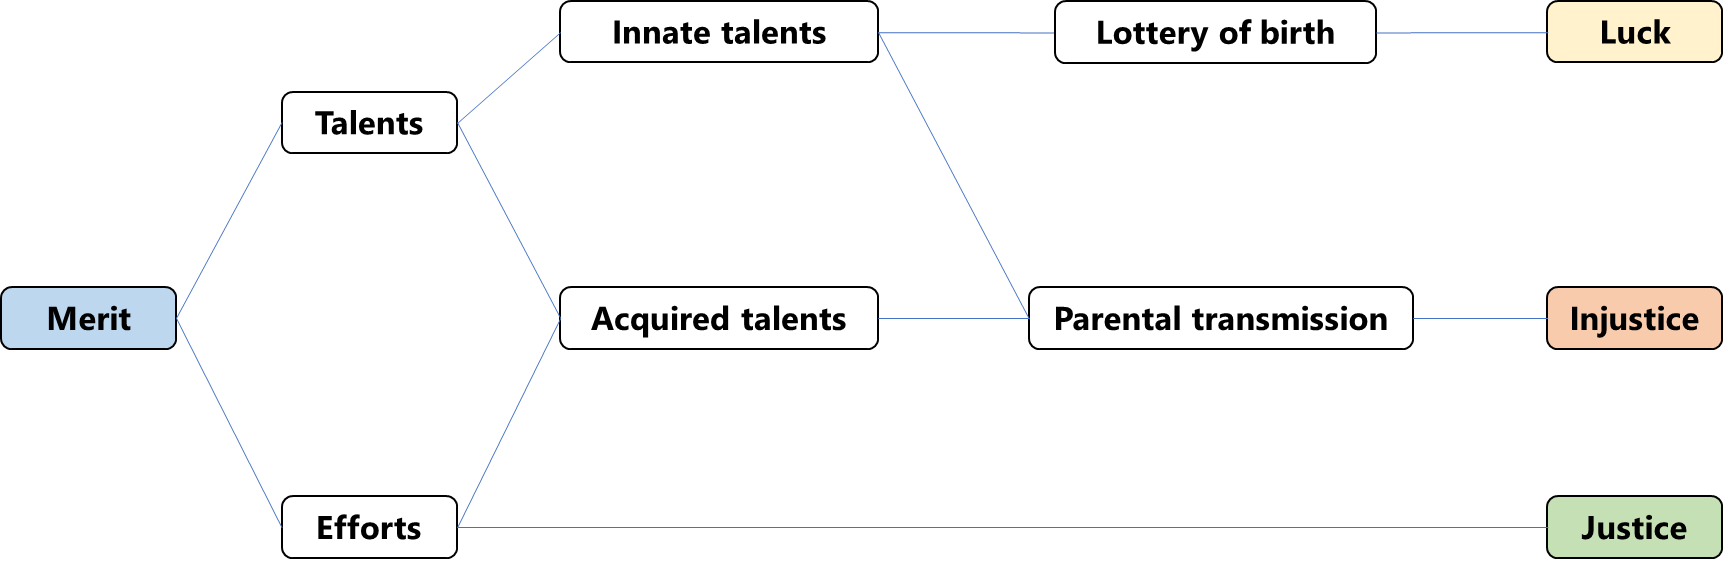
\includegraphics[width=0.9\linewidth]{figs/fig1}
	\caption{Merit = talent + effort}
	\label{fig:fig1}
	\begin{minipage}{1\linewidth}
		\vspace{0.2cm}
		\footnotesize
		\textbf{Notes:} Merit, typically a blend of talent and effort, connects effort to justice, but the link between talent and justice is intricate. Talents split into two types: innate and acquired. Innate talents emerge from the birth lottery, akin to luck in parental inheritance. In contrast, acquired talents demand strenuous learning and training, influenced by personal aptitude and parental investment in education and upbringing. Parental transmission, particularly in socioeconomic aspects, is often seen as unjust.
		
		\textbf{Source:} The author(s)
	\end{minipage}
\end{figure}

Another issue with defining merit lies in the concept of effort. Merit is often defined as intelligence plus effort, but how is effort measured when identifying merit at an early age? For the working class, meritocracy represents hope, and their only advantage over other classes is their effort or hard work. This class did not inherit natural intelligence from their parents and did not receive educational investment from their parents due to economic constraints. The demarcation between effort and talent is frequently overlooked, predicated on the assumption that the exertion of effort is inherently encapsulated within the resultant outcomes \citep{dunlosky2020role}. This viewpoint, however, conspicuously neglects the role of luck. As posited by scholar Michael \citet{shermer2017secret}, success is an amalgamation of talent, effort, and luck. This leads us to the critical inquiry:

\begin{question} \label{q1}
	Does the belief in meritocracy retain its validity when the significance of effort is diminished?
\end{question}

\subsection{Materials and methods (Study 1)}

To investigate the validity of the meritocracy belief (Question~\ref{q1}), Boolean analysis was employed to assess the logical coherence of the principles advocated by a meritocratic system. This method, while not entirely novel, originates from propositional calculus or statement logic \citep{buning1999propositional}. It operates within the realm of propositions, which are statements that can be either true or false, and their interrelations, which form the basis for constructing arguments. An argument consists of two components: a set of statements known as premises, and a single statement termed the conclusion. The conclusion is posited to logically follow from the premises, which are purported to provide support for the conclusion. The statements are commonly analyzed by replacing atomic (indivisible) statements with alphabet letters, which are interpreted as variables representing statements (propositional variables). Thus, in this study, the logical coherence of the meritocratic argument was assessed by formalizing the premises of meritocracy into propositional variables, in order to deduce the conclusion that meritocracy is just. In other words, meritocracy is logically just if and only if the meritocratic argument always holds true, constituting a tautology.

Here, I construct a statement comprising four premises \nameref{H1}--\nameref{H4} and one conclusion \nameref{Q} 
(see the definition of components in Table~\ref{tab:tab1}).

\begin{premise*}[H1]\label{H1}
	$
	L \Rightarrow (G \cap N) \quad \text{or} \quad L \Rightarrow (G \cup N).
	$
	The emergence of talent can be attributed to an amalgamation of inherent characteristics and nurtured competencies, or it may be exclusively derived from either of these constituents. The former proposition underscores the pivotal role of genetic predispositions in talent manifestation, while the latter advocates for the potential of talent evolution independent of genetic constraints, facilitated by dedicated learning and practice. This dichotomy forms the crux of the perennial nature versus nurture discourse pertaining to the development of abilities \citep{meyer2022talents}.
\end{premise*}

\begin{premise*}[H2]\label{H2}
	$
	G \Rightarrow P \quad \text{or} \quad (G \Rightarrow P) \cap (G \Rightarrow J).
	$
	The attainment of success can be attributed to the acquisition of superior genetic traits from one’s progenitors. This perspective is often viewed as a matter beyond human influence as natural inequality \citep{aas2016natural}, while some interpret it as a manifestation of fortuitous circumstances, devoid of any notions of justice or injustice. This premise is relevant to the discussions on luck egalitarianism \citep{knight2013luck}.
	
\end{premise*}

\begin{premise*}[H3]\label{H3}
	$
	N \Rightarrow (P \cup L) \cap O.
	$
	The process of acquiring educational credentials or mastering skills can be accelerated by parental aid, such as financial support for international studies, or through an individual’s pre-existing expertise \citep{meyers2013talent}, such as someone with a foundation in Information Technology effortlessly gaining more IT-related skills. Nonetheless, this theory must also factor in the role of personal diligence. Irrespective of the degree of parental contribution or backing, the fruits of education and training cannot be reaped without the individual’s commitment and allocation of time.
	
\end{premise*}

\begin{premise*}[H4]\label{H4}
	$
	(O \Rightarrow J) \cap (P \Rightarrow \bar{J}).
	$
	In societal constructs, the perception of fairness often dictates that success achieved through personal effort is considered meritorious, while success derived from inheritance is not viewed with the same level of esteem \citep{rowlingson2011deserving}.
	
\end{premise*}

\begin{conclusion*}[Q]\label{Q}
	$
	(M = L) \Rightarrow J \quad \text{or} \quad (M = L \cap O) \Rightarrow J.
	$
	This proposition is based on the scenario where effort is undervalued in the process of assessing merit. The first scenario emphasizes that talent is the essence of merit, while the second scenario suggests that talent and effort have equal importance. However, as per the belief in meritocracy, regardless of the metric used, the concept of merit cannot be solely equated with hard work \citep{clavero2023idea}. In this context, hard work merely serves as a mechanism for individuals to compensate for lower levels of talent, thereby emphasizing the importance of acknowledging one’s limitations determined by talent (abilities, skills, and expertise), as argued by \citet{chamorro2016talent}.
	
\end{conclusion*}

Table~\ref{tab:tab1} presents a comprehensive overview of the eight distinct scenarios concerning the belief in meritocracy. Subsequently, a Boolean algebraic methodology is employed to analyse the logical constructs associated with meritocracy belief (see details in \ref{app:boolean}).

\begin{sidewaystable}
\begin{table}[H]
	\centering
	\caption{Is the belief in meritocracy true?}
	\label{tab:tab1}
	\renewcommand{\arraystretch}{1.4}
	\resizebox{\textwidth}{!}{%
	\begin{tabular}{c|c|c|c|c|c|c}
		\textbf{\#} & \textbf{\nameref{H1}} & \textbf{\nameref{H2}} & \textbf{\nameref{H3}} & \textbf{\nameref{H4}} & \textbf{\nameref{Q}} & \textbf{\nameref{H1} $\cap$ \nameref{H2} $\cap$ \nameref{H3} $\cap$ \nameref{H4} $\Rightarrow$ \nameref{Q}} \\
		\hline
		1 & $L \Rightarrow G \cup N$ & $G \Rightarrow P$ & $N \Rightarrow (P \cup L) \cap O$ & $(O \Rightarrow J) \cap (P \Rightarrow \bar{J})$ & $(M = L) \Rightarrow J$ & $G \cap \bar{N} \cap L \cap P \cap \bar{O} \Rightarrow J$ \\
		2 & $L \Rightarrow G \cup N$ & $(G \Rightarrow P) \cap (G \Rightarrow J)$ & $N \Rightarrow (P \cup L) \cap O$ & $(O \Rightarrow J) \cap (P \Rightarrow \bar{J})$ & $(M = L) \Rightarrow J$ & Tautology \\
		3 & $L \Rightarrow G \cup N$ & $G \Rightarrow P$ & $N \Rightarrow (P \cup L) \cap O$ & $(O \Rightarrow J) \cap (P \Rightarrow \bar{J})$ & $(M = (L \cap O)) \Rightarrow J$ & Tautology \\
		4 & $L \Rightarrow G \cup N$ & $(G \Rightarrow P) \cap (G \Rightarrow J)$ & $N \Rightarrow (P \cup L) \cap O$ & $(O \Rightarrow J) \cap (P \Rightarrow \bar{J})$ & $(M = (L \cap O)) \Rightarrow J$ & Tautology \\
		5 & $L \Rightarrow G \cap N$ & $G \Rightarrow P$ & $N \Rightarrow (P \cup L) \cap O$ & $(O \Rightarrow J) \cap (P \Rightarrow \bar{J})$ & $(M = L) \Rightarrow J$ & Tautology \\
		6 & $L \Rightarrow G \cap N$ & $(G \Rightarrow P) \cap (G \Rightarrow J)$ & $N \Rightarrow (P \cup L) \cap O$ & $(O \Rightarrow J) \cap (P \Rightarrow \bar{J})$ & $(M = L) \Rightarrow J$ & Tautology \\
		7 & $L \Rightarrow G \cap N$ & $G \Rightarrow P$ & $N \Rightarrow (P \cup L) \cap O$ & $(O \Rightarrow J) \cap (P \Rightarrow \bar{J})$ & $(M = (L \cap O)) \Rightarrow J$ & Tautology \\
		8 & $L \Rightarrow G \cap N$ & $(G \Rightarrow P) \cap (G \Rightarrow J)$ & $N \Rightarrow (P \cup L) \cap O$ & $(O \Rightarrow J) \cap (P \Rightarrow \bar{J})$ & $(M = (L \cap O)) \Rightarrow J$ & Tautology \\
	\end{tabular}
}
	\begin{minipage}{1\linewidth}
		\vspace{0.2cm}
		\footnotesize
		\textbf{Notes:} 
		G = ‘Success comes from innate talent’; L = ‘Success stems from individual talent’; P = ‘Success is attributed to parental inheritance’; N = ‘Success is a result of learning and training processes’; O = ‘Success is achieved through effort’; M = ‘Success is earned based on merit’; J = ‘Success is deserved’.
		
		\textbf{Source:} The author(s)
	\end{minipage}
\end{table}

\end{sidewaystable}

\subsection{Results and Discussion (Study 1)}

As depicted in Table~\ref{tab:tab1}, the belief in meritocracy can be justified through the exertion of effort or hard work, as evidenced by Scenarios 3, 4, 7, and 8. This is a logical assertion since even individuals who possess favourable circumstances, such as coming from a wealthy family, cannot achieve deserving success without putting forth effort in their studies and work. Similarly, the recognition that talents can be acquired through training without innate factors, such as certain types of physical skills that do not rely on genetics and only through hard training, would also justify beliefs in meritocracy, as evidenced by Scenarios 5, 6, 7, and 8. These scenarios are tautologies. In instances where the evaluation of merit does not incorporate effort, as evidenced in Scenarios 1 and 2, beliefs in meritocracy are only valid if difference legitimation ($G \implies J$) is present. This necessitates those innate talents be considered just, as indicated by Scenario 2. Hence, investigations into the belief in meritocracy and its relationship to social justice ought to centralize around three fundamental aspects: (1) Scrutinizing whether innate talents (and factors beyond human influence) are deemed as fair or merely the result of luck; (2) Exploring whether merit is perceived as obligatory, constrained, or potentially disconnected from an individual's genetic makeup or biological influences; (3) Determining whether the inclusion of effort and diligence is an obligatory component in assessing an individual's merit.

First, this study contributes to the argument for luck egalitarianism against meritocracy. Innate talent is heavily influenced by genetic factors, thus, it can be considered a product of the lottery of birth \citep{mijs2022earning}. Each individual is born with varying abilities, such as intelligence. These natural differences between individuals can result in differences in social value when viewed through a societal lens. As this is beyond human control, the lottery of birth can be considered just, albeit controversial \citep{aas2016natural}. However, it is not inherently unjust. Furthermore, inherent talents are often a product of one’s lineage. Parents who are intelligent and well-off are more likely to transmit their beneficial genes to their children \citep{mijs2022earning}. This is no different from inheriting socioeconomic advantages from one’s parents, which is often considered undeserved and unjust \citep{rowlingson2011deserving}. In a meritocratic society, these children are afforded better opportunities. This perpetuates inequality, as the wealthy and intelligent continue to accumulate wealth and intelligence, known as the Matthew Effect~\citep{bask2015cumulative}. This process mirrors the widening income gap between the rich and the poor.

The second contribution of this study is to the ongoing nature versus nurture debate. Acquired talent, unlike innate talent, can be developed through various means. These include parental guidance, investment in early childhood education, and the pursuit of new skills or qualifications in adulthood. However, the acquisition of such talent necessitates a process of learning and training, which requires both time and effort. Knowledge and skills, being intangible assets, cannot be easily transferred like tangible assets such as money or property. Instead, they must be acquired through a dedicated process of learning and training~\citep{meyers2013talent}. Based on the above Boolean analysis, the perception of whether talents can be developed based solely (or largely) on individual effort is crucial to establishing a fair meritocracy. Therefore, there is a pressing need for scientific evidence to clarify this viewpoint. This evidence would provide a more nuanced understanding of talent development and its implications for societal structures and norms.

Lastly, challenging the naturalness bias, this research advocates for the inclusion of a separate evaluation criterion for effort to ensure the fairness and rationality of the meritocratic system. Effort plays a pivotal role in social fairness and forms the foundation for the majority of society’s aspirations for advancement. This research supports Robert~\citeauthor{marzano2000transforming}’s viewpoint that effort should be taken into account when assessing a student’s performance. In a meritocratic society, where equality of opportunity is emphasized and opportunities are allocated to individuals based on their talents, it raises the question of how individuals from working-class backgrounds can ascend to higher social classes. These individuals often possess only one asset: their effort. In their pursuit of opportunity, they may be required to exert significantly more effort than their more talented counterparts. This highlights the need for a meritocratic system that recognizes and rewards effort, thereby promoting social mobility and reducing inequality.

\section{The paradox of privilege in meritocratic justice}

\epigraph{In its quest for justice, meritocracy paradoxically nurtures the notion of privilege, the very cornerstone of injustice, by emphasizing equal opportunities.}{The author}

We are confronted with an ever-widening chasm between the affluent and the impoverished, and we are in search of remedies to diminish it. This is not solely due to it being the fundamental cause of a plethora of societal and environmental issues~\citep{harlan2015climate}, but also because it is a manifestation of injustice. Not all wealth is attained through diligence and perseverance. While numerous individuals endeavour to ascend in society through education and hard work, some inherit wealth from their progenitors without exerting any effort. Furthermore, social stereotypes pertaining to gender, ethnicity, and social class persist and can dictate an individual’s destiny. To address this quandary, progressive societies such as those in the US and UK have established a meritocracy where talent and effort are rewarded~\citep{soares2017meritocracy}. In a democratic society where the majority of the working class is still striving for social mobility, meritocracy represents their hope and justice. However, we did not anticipate that meritocracy would become a valid justification for social stratification and increasing inequality~\citep{markovits2019meritocracy} – a problem it should have resolved. Indeed, research by Jonathan~\citet{mijs2021paradox} shows that belief in meritocracy goes hand in hand with income inequality, using International Social Survey Program data.

Perhaps the crux of this conundrum lies not in the dichotomy between income equality and meritocracy, but in social fairness and opportunity equality. We are not advocating for radical income equality, but rather for social fairness, where those who exert greater effort should receive commensurate rewards~\citep{starmans2017people}. We do not require a convoluted meritocracy, but rather a straightforward equality of opportunity where everyone has the chance to develop themselves and achieve success~\citep{swift1997meritocratic}. Thus, while belief in meritocracy and income inequality go hand in hand,

\begin{question}
	Does meritocratic opportunity equality indeed go hand in hand with social fairness?
\end{question}

\subsection{Materials and Methods (Study 2)}
Our objective is to champion social fairness, but what does this fairness encompass? It might be reflected in hardworking individuals earning more than others, a belief in meritocracy shared by most of the working class. Alternatively, it could involve supporting the impoverished and those in need. It might even advocate for equal income and wealth distribution, or perhaps even privileges for individuals from high social standing families. The 9th European Social Survey (ESS-9) survey indicates that society largely agrees that hardworking people should earn more, and that support should be provided for the impoverished and needy (refer to Figure~\ref{fig:fig2}). Some also advocate for equal income and wealth distribution, but most disagree with privileges for individuals from high-social-status families (though this belief persists). Each aspect of social fairness may represent a unique form of distributive justice within society~\citep{hulle2018measuring}: ‘Equality’ (equal distribution of goods and burdens), ‘Need’ (allocation based on basic needs), ‘Equity’ (distribution based on individual contributions), and ‘Entitlement’ (distribution based on status and past achievements). It can be seen that among the four distributive justice principles, ‘Equity’ is strongly associated with the belief in meritocracy, which holds that those who work harder deserve greater rewards. Hereafter, I will refer to ‘Equity’ as meritocratic fairness.

\begin{figure}[h!]
	\centering
	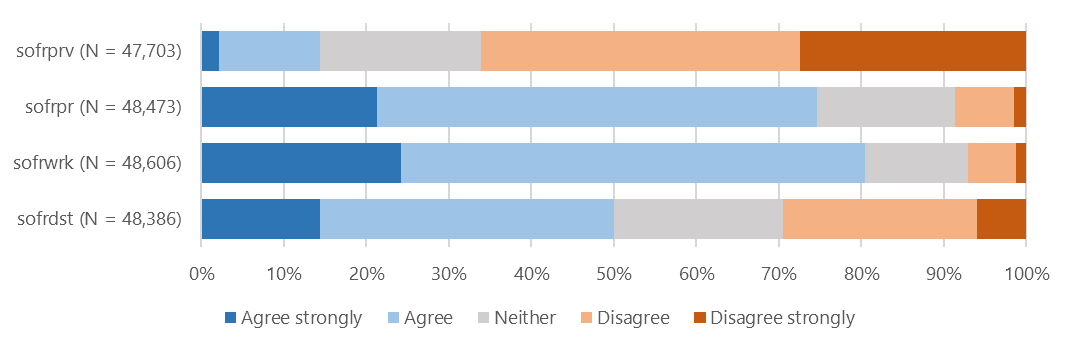
\includegraphics[width=0.9\linewidth]{figs/fig2}
	\caption{Social Fairness across European countries}
	\label{fig:fig2}
	\begin{minipage}{1\linewidth}
		\vspace{0.2cm}
		\footnotesize
		\textbf{Notes:}	The data, sourced directly from the 9th round of the European Social Survey (ESS-9), provides insights into societal fairness perceptions. The variables include equal distribution of income and wealth (\texttt{sofrdst}), reward for hard work (\texttt{sofrwrk}), support for the poor and needy (\texttt{sofrpr}), privileges for high social status (\texttt{sofrprv}).	
	\end{minipage}
\end{figure}


In this research, meritocracy is conceptualized as being synonymous with equality of opportunity. The perception of meritocracy is measured by evaluating viewpoints on elements that influence recruitment decisions, which are also seen as opportunities. According to the ESS-9 survey (see Figure~\ref{fig:fig3}), there are five fundamental categories of elements that affect opportunities: (1) gender, (2) immigrant background, (3) knowing someone in the organization, (4) on-the-job experience, and (5) knowledge and skills. Notably, the fourth and fifth categories exhibit a robust correlation with the conviction in meritocracy, which posits that opportunities are allocated to deserving individuals predicated on their merit. Henceforth, I will denote hiring decisions predicated on such work experience and competencies as meritocratic equality of opportunities.

\begin{figure}[h!]
	\centering
	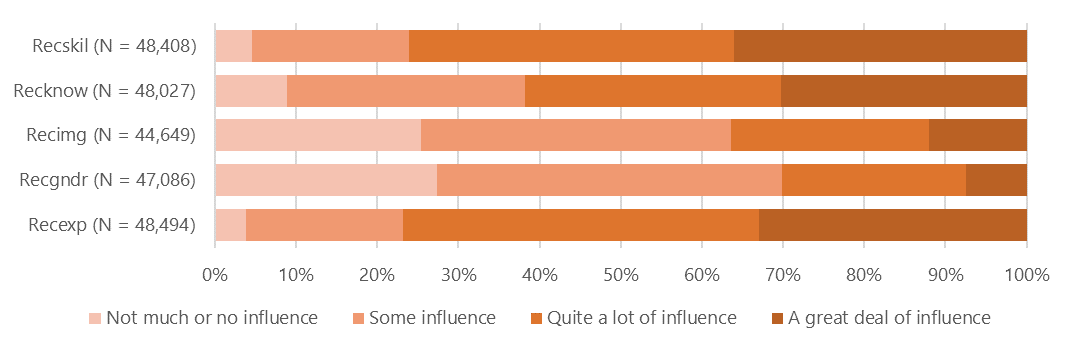
\includegraphics[width=0.9\linewidth]{figs/fig3}
	\caption{Opportunity equality across European countries}
	\label{fig:fig3}
	\begin{minipage}{1\linewidth}
		\vspace{0.2cm}
		\footnotesize
		\textbf{Notes:}	The data provided is sourced from the 9th round of the European Social Survey (ESS-9). It includes several factors that influence the decision to recruit a person in a country. These factors are on-the-job experience (\texttt{recexp}), gender (\texttt{recgndr}), immigrant background (\texttt{recimg}), knowing someone in the organization (\texttt{recknow}), and knowledge and skills (\texttt{recskil}).	
	\end{minipage}
\end{figure}

The concepts of social fairness and equality of opportunity are indeed complex and can be interpreted differently, often influenced by one’s cultural, societal, and personal beliefs~\citep{trautmann2023procedural}. Therefore, providing a specific principle to evaluate social fairness or opportunity equality is challenging. A significant advancement of this research is the intentional avoidance of enforcing any principle of distributive justice as the optimal outcome, and similarly for opportunity equality. This approach acknowledges that these measures are inherently biased to a certain extent and could be swayed by subjective interpretations of social fairness and equality of opportunity. In order to evaluate social fairness and opportunity equality in accordance with democratic principles, this study focuses on the preferences of the majority population. This is accomplished by creating a universal scale for each factor, using the unidimensional scaling method detailed later. Consequently, this research transcends the limitations imposed by a rigid definition of social fairness or equality of opportunity, allowing the empirical data to accurately represent the collective desires of the societal majority.

This study employs data from the 9th round of the European Social Survey, which was conducted in 2018 and focused on the Timing of Life, Justice, and Fairness. The cleaned data consists of 454 individuals and 56 variables (see details of the cleaning process in \ref{app:cleaning}). To detect possible relationships among variables, I proceeded to employ clustering techniques commonly used in the study of genes, wherein the variables representing social fairness and opportunity equality are treated as ‘genes’ with distinct characteristics that form high-dimensional data. The problem of social fairness thus becomes one of clustering such ‘genes.’ Due to the immense computational requirements and in order to visualize the results, I reduced the dimensionality of these ‘genes’ into a 2-dimensional space while ensuring that as much dissimilarity information between them was retained. The clustering results would be robust due to the comparison of clustering techniques and bootstrapping of data (see details in \ref{app:clustering}).

Prior to conducting clustering analysis, a selection of variable sets that exhibit a strong correlation with social fairness and opportunity equality was made based on previous research:

\begin{itemize}

\item The ‘government performance’ group includes five variables assessing views on democracy, government performance, national economy, health services, and education system as~\citet{ruger2020social} study shows the relationship between social justice, democracy, and health.

\item The 'discrimination' group includes seven variables indicating aspects like gender and citizenship, while the 'socioeconomic status' group has 11 variables related to income, education, and occupation. Discriminatory behaviours can arise from factors like education, social class, and political beliefs among powerful individuals~\citep{bhugra2016social}.

\item The ‘social trust’ group contains three variables that convey personal sentiments about social trust and interactions between people in society as~\citet{carter2016microsociologies} contends that these variables are interrelated with social justice.

\item The ‘human values’ group is composed of 21 variables that assess the significance of various human values to respondents. This group is derived from the study by ~\citet{tittler2020personal}, which discovered that personal values matter to social fairness.

\end{itemize}

\begin{figure}[h!]
	\centering
	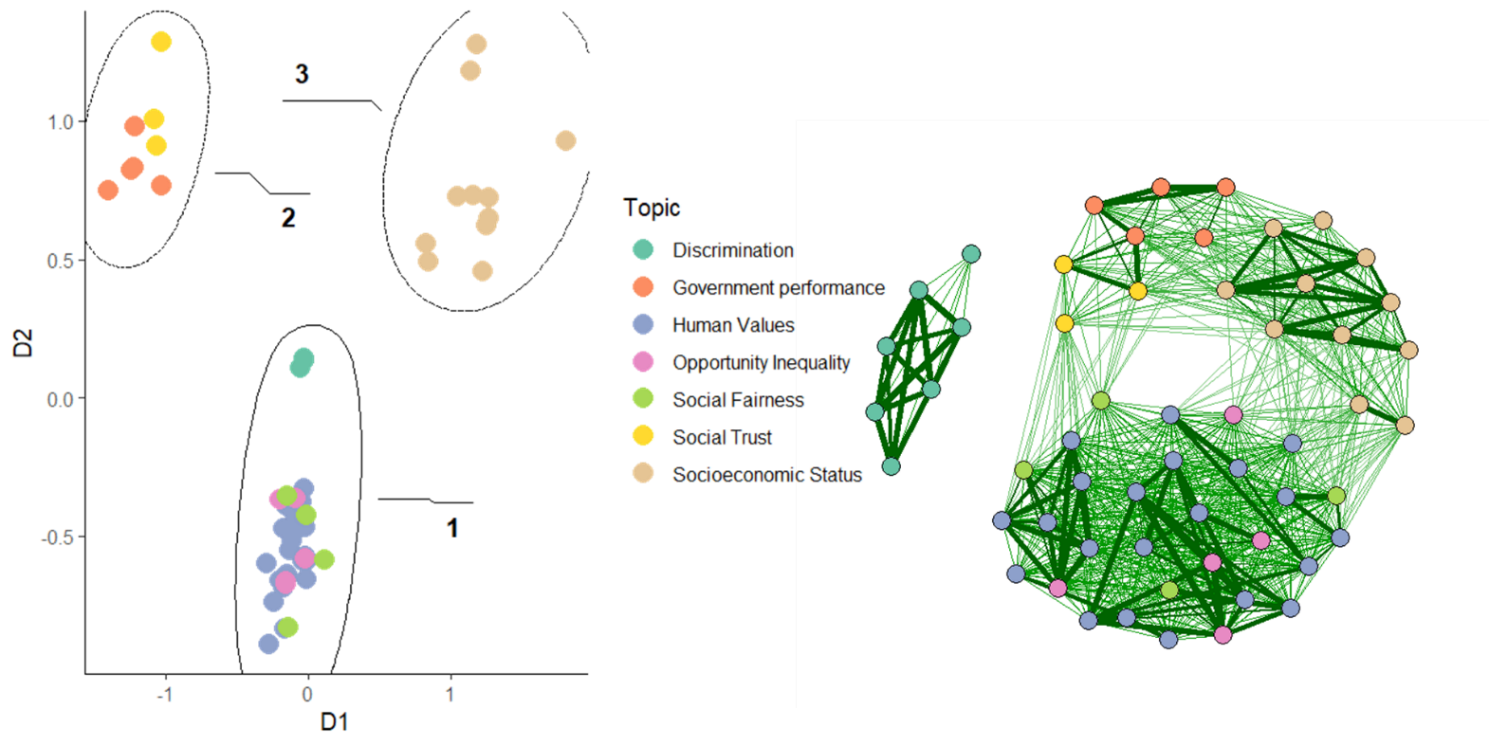
\includegraphics[width=1\linewidth]{figs/fig4}
	\caption{Which relates to the belief in social fairness?}
	\label{fig:fig4}
	\begin{minipage}{1\linewidth}
		\vspace{0.2cm}
		\footnotesize
		\textbf{Notes:}	The data utilized in this figure is the unfolded data of the European Social Survey Round 9 (comprising 454 individuals and 56 variables). The clusters depicted in the graph are generated using the K-means clustering algorithm. The correlation network reports only correlation coefficients with absolute values greater than 0.5.
	\end{minipage}
\end{figure}

The cluster analysis, as depicted in Figure~\ref{fig:fig4}, indicates that characteristics of discrimination, including gender and migration background, exhibit similarities with social fairness, equality of opportunity, and human values due to their co-location within the same cluster. Despite this, a lack of connection between these discrimination characteristics and the aforementioned traits is observed in the correlation network. Conversely, variables related to socioeconomic status, government performance, and social trust do not belong to the same cluster as fairness beliefs but demonstrate a close association with them. This implies that discrimination status could serve as a determinant for identifying cohorts with analogous fairness belief perceptions. Nonetheless, alterations in fairness beliefs necessitate modifications in socioeconomic status, government performance, and social trust. A study conducted by~\citet{bakhtiari2022diminished} using European Social Survey data found evidence of diminished returns (on their investments in human capital, such as education and income) for minority populations originating from Sub-Saharan Africa and the Middle East. This suggests that an immigration background can serve to identify groups of individuals with similar experiences of social fairness. This finding also aligns with the persistent race and gender inequality in society, where those experiencing such disparities strive for social fairness~\citep{becares2015understanding}.

\subsection{Results and Discussion (Study 2)}

In this study, I aim to measure the social fairness that the majority of society believes in a certain dimension when the definition of it is not entirely feasible. Even though ‘Equity’ (which is strongly associated with belief in meritocracy) is widely agreed upon (as per the ESS-9), it does not mean that meritocracy is a means of justice.
By employing unidimensional scaling, I transform four-dimensional social fairness into one-dimensional social fairness while removing personal preferences and unfolding ordinal data as commonly employed in psychological science (see details in \ref{app:uniscale}). It should be observed that variations in institutional factors, such as country-specific characteristics, cultural context, and social norms, are manifested in individual preferences. Consequently, this methodology is applicable to the analysis of cross-national data within the EU context.

The unidimensional scaling results (see the scale charts in Figure~\ref{fig:fig5}) show that, as expected, \texttt{sofrwrk} and \texttt{sofrprv} have the largest value of 0.65 and the smallest value of -0.938 on the social fairness scale, respectively. The negative sign of \texttt{sofrprv} shows people generally against Entitlement as social unfairness. Similarly, with the unidimensional scale for the factors that influence recruitment decisions, the estimated results will yield a measure of bias in recruitment decisions, or in other words, opportunity inequality. This scale shows that \texttt{recskil} and \texttt{recexp} have the smallest values of -0.663 and -0.636 while \texttt{recgndr} and \texttt{recimg} occupy the top two positions of 0.818 and 0.671. The negative signs of \texttt{recskil} and \texttt{recexp} suggest a perception of opportunity equality rather than inequality. These findings are not surprising at all, suggesting that meritocratic factors represent both social fairness and opportunity equality. However, it is premature to conclude that meritocratic equality of opportunities goes hand in hand with meritocratic fairness.

\begin{figure}[h!]
	\centering
	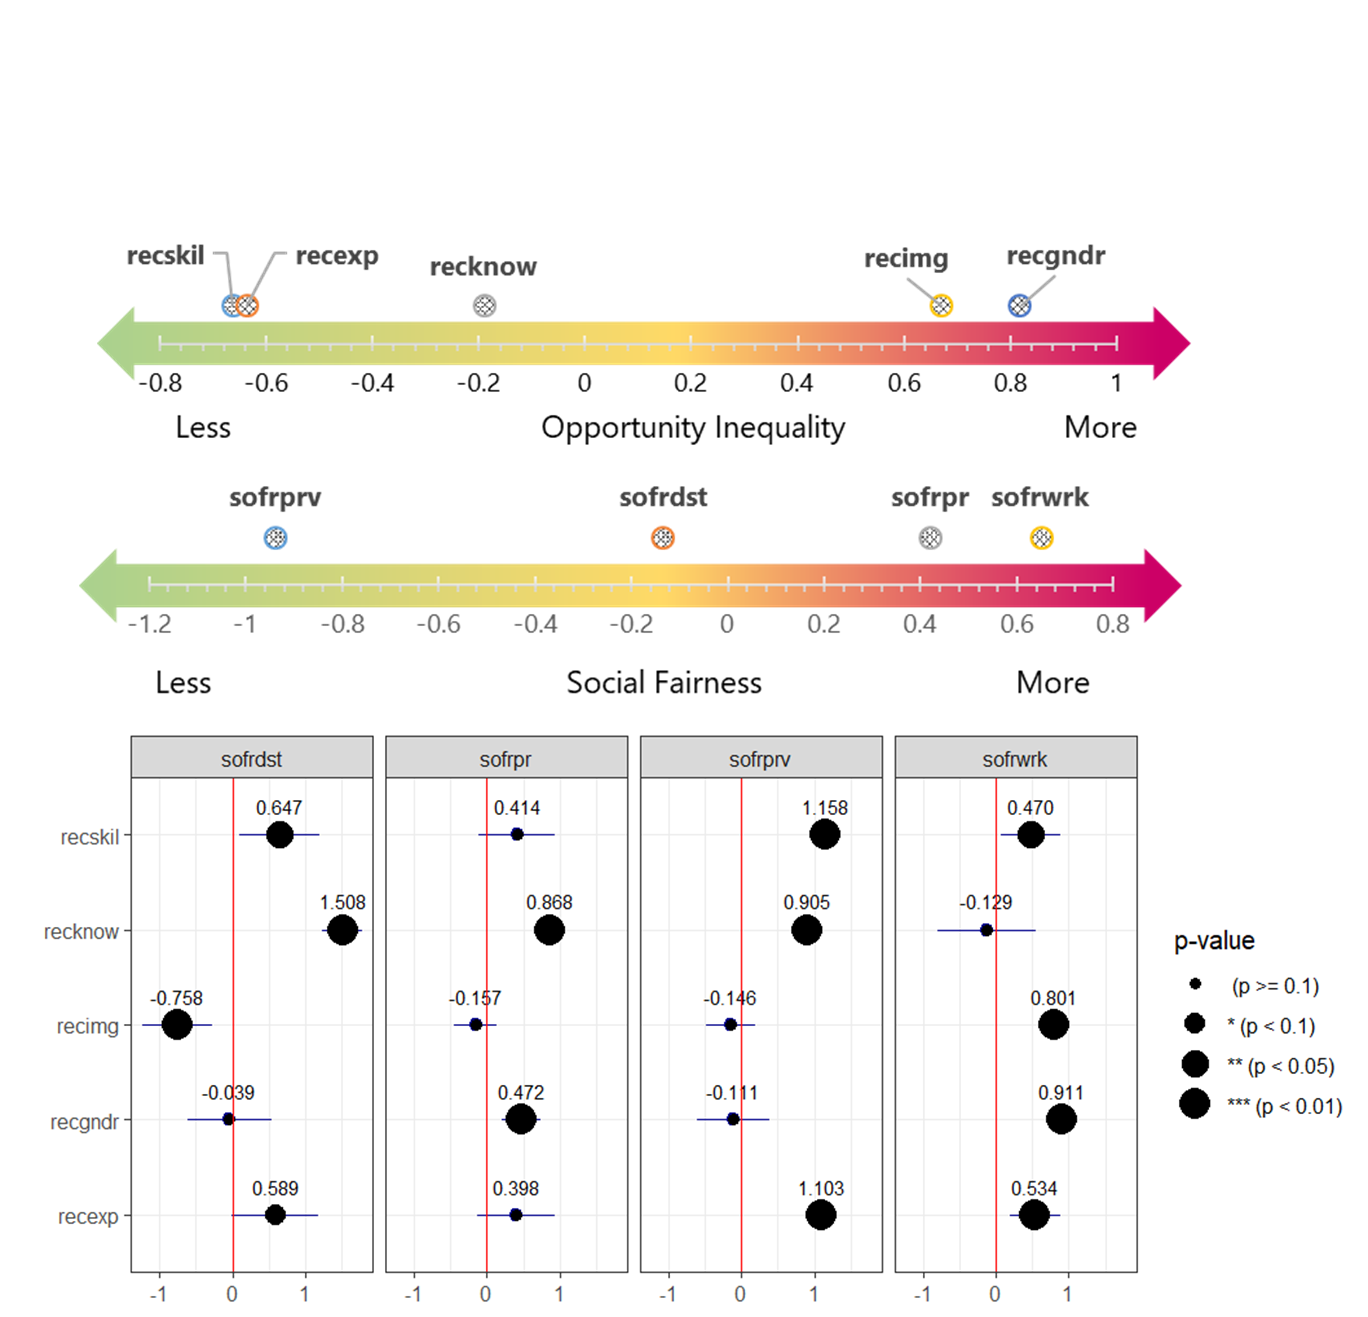
\includegraphics[width=1\textwidth]{figs/fig5.png}
	\caption{Does opportunity equality translate into social fairness?}
	\label{fig:fig5}
		\begin{minipage}{1\linewidth}
		\vspace{0.2cm}
		\footnotesize
		\textbf{Notes:}	The data utilized in this figure is the unfolded data of the European Social Survey Round 9 (comprising 454 individuals and 56 variables). The two scale charts employ the unidimensional scaling technique. The estimated plot utilizes the double machine learning technique, where row names represent independent variables and column names represent dependent variables. The effect of each pair of independent and dependent variables is estimated separately, resulting in a total of 20 estimates. These estimators are comparable because they share the same scale.
	\end{minipage}
	
\end{figure}

By further harnessing the power of the double machine learning analysis technique with robustness through cross-validation by K-folds (see details in \ref{app:kfold}) in the realm of computer science, I was able to accurately estimate the ‘pure’ effects of opportunity equality on social fairness, while adeptly addressing confounding problems and multicollinearity in social science (using unfolded data). 
The results of my meticulous estimation (see Figure~\ref{fig:fig5}) yielded solid evidence that meritocratic equality of opportunities does not go hand in hand with meritocratic fairness, but rather with a belief in privileges. The meticulous analysis reveals that the variables \texttt{recskil} and \texttt{recexp}, indicative of meritocratic equality of opportunities, exert a somewhat indistinct influence on \texttt{sofrwrk}, a measure of meritocratic fairness, with effect sizes of 0.470 and 0.534 respectively. However, these variables demonstrate a substantial impact on \texttt{sofrprv}, a representation of belief in privilege, with effect sizes of 1.158 and 1.103 respectively. Conversely, the variables \texttt{recimg} and \texttt{recgndr}, which show non-meritocratic equality of opportunities still exists, promote the belief in a fair society based on hardwork (\texttt{sofrwrk}) with effect sizes of 0.801 and 0.911. Furthermore, \texttt{recknow}, a variable representing relationship advantages, also exerts a noteworthy influence on \texttt{sofrprv} with an effect size of 0.905. Ironically, beliefs in social fairness that benefit underprivileged people, such as ‘Equality’ or ‘Need’, are hardly promoted by meritocratic equality of opportunities. As depicted in Figure~\ref{fig:fig5}, \texttt{sofrdst} and \texttt{sofrpr} are not influenced by \texttt{recskil} and \texttt{recexp} due to statistically insignificant effects or large estimate errors. Instead, they are influenced by \texttt{recknow} (non-meritocratic equality of opportunities) with effect sizes of 1.508 and 0.868 respectively.

These findings unveil a paradox: while the working class endeavours for equal opportunities, it results in a perception of distributive unfairness where individuals from higher social classes relish privileges. This paradox completely coincides with observation and interview data in St. Paul's School in the US by~\citet{khan2013saying}. They stated, ``the elite saying meritocracy but doing the ease of privilege''. The qualitative study by ~\citet{nahai2013meritocracy} on admissions at the University of Oxford previously suggested that disparities in admissions outcomes in elite universities among various social groups, often perceived as unfair or biased towards socially privileged applicants, are in fact a reflection of societal inequality. This inequality manifests in the correlation between academic achievement and factors such as social class and family income. It is evident that meritocracy has served to legitimize social inequality and rationalize the wealth of affluent individuals on the basis of their superior merits. Pierre~\citet{bourdieu2017sociologie} once argued that ``the school plays one of the most important roles in the reproduction of social inequalities with the help of the symbolic violence present in every pedagogical act, particularly when it functions as the legitimate agent of society''~\citep{tavsner2022time}.

In \textit{The Meritocracy Trap}, Daniel~\citet{markovits2019meritocracy} explains these meritocratic inequalities through a two-step process. Firstly, elite workers displace middle-class workers from key economic roles due to their high skills. Secondly, these elites use their wealth to provide superior education for their children, giving them an edge in high-skilled sectors. This leads to ``snowball inequality'', a self-reinforcing cycle that intensifies economic disparity, limits social mobility, and creates a ``time divide'' between overworked elites and an increasingly idle middle class. In a meritocratic society where talent and effort are esteemed, most of the individuals who reap the benefits of this system are those from privileged backgrounds with access to quality education. This is far removed from the reality for impoverished classes that rely solely on the public education system. We have employed meritocracy as a panacea for the inequality malady of society, but it has transpired to be a poison.

This study presents robust quantitative evidence supporting the existence of a meritocracy trap, akin to the poverty trap, where an individual's low income inhibits investment in education or other forms of self-improvement, thereby perpetuating their impoverished state. In contemporary society, meritocratic equality of opportunity was conceived as a mechanism to mitigate social inequalities, offering fair conditions for disadvantaged individuals to ascend socio-economic ranks based on a merit-based system. However, disadvantaged individuals often lack the competitive merits possessed by their privileged counterparts to seize such opportunities. Consequently, such meritocratic equality of opportunity inadvertently reinforces beliefs in privilege, thereby perpetuating social stratification. Based on the scientific evidence in this study, I support the view that we need to ensure a radical rather than meritocratic equality of opportunity~\citep{segall2013equality}, especially in the field of education.

\section{Conclusion}

This study aimed to investigate the question of whether meritocracy is just by conducting two distinct inquiries to gain comprehensive insights into the complexities of this concept. The first inquiry using Boolean analysis shows ‘the paradox of hard work in a meritocracy: While meritocracy is a beacon of justice, it ironically undervalues hard work, the very architect of fairness, in favour of talent’. This finding contributes to ongoing debates against the current belief in meritocracy. This study identifies three conditions (not necessarily simultaneous) to construct the rationality of meritocracy: First is difference legitimation when merit is just the result of luck (as per luck egalitarianism). Second is that genes should not limit one’s ability as per the nature-nurture debate. Third is that effort should be the score at evaluating merit (against the naturalness bias). The second inquiry using machine learning approaches shows ‘the paradox of privilege in meritocratic justice: In its quest for justice, meritocracy paradoxically nurtures the notion of privilege, the very cornerstone of injustice, by emphasizing equal opportunities.’ This finding strengthens the argument that belief in meritocracy goes hand in hand with inequality when meritocratic equality of opportunities goes hand in hand with privileges. This conclusion interestingly relates to observations by \citet{khan2013saying} at St. Paul’s School in the US. He argues that the elite say meritocracy but practice privilege. In conclusion, this study contributes useful insights to build a new meritocracy that \citet{tavsner2022time} is advocating for. This new meritocracy should ensure fairness from the early stages of children's lives.

\printbibliography[heading=subbibliography]

\begin{appendices}
	\renewcommand{\thesection}{Appendix \arabic{section}}

\small

\newpage
\section{Boolean analysis} \label{app:boolean}
To simplify the interpretation of the Boolean algebraic calculation, I replaced the logical symbols with the following substitutions: \(X \implies Y\) became \(X \to Y\); \(X \cap Y\) became \(X \cdot Y\); \(X \cup Y\) became \(X + Y\), and \(\overline{X}\) is the negation of \(X\). I commence with Scenario 4:
\[
\big((L \to (G + N)) \cdot (G \to J) \cdot (G \to P) \cdot (N \to ((P + L) \cdot O)) \cdot (O \to J) \cdot (P \to \overline{J})\big) \to (L \cdot O \to J)
\]
Applying the equivalence \(X \to Y = \overline{X} + Y\) to each premise and the conclusion then the entire statement, the expression is transformed to:
\[
\big((\overline{L} + G + N) \cdot (\overline{G} + J) \cdot (\overline{G} + P) \cdot (\overline{N} + ((P + L) \cdot O)) \cdot (\overline{O} + J) \cdot (\overline{P} + \overline{J})\big)^{\overline{}} + \big((L \cdot O)^{\overline{}} + J\big)
\]
Further utilizing the equivalence \((X \cdot Y)^{\overline{}} = \overline{X} + \overline{Y}\) for the entire statement, and subsequently applying \((X + Y)^{\overline{}} = \overline{X} \cdot \overline{Y}\) to each premise, we obtain the expression:
\[
L \cdot \overline{G} \cdot \overline{N} + G \cdot \overline{J} + G \cdot \overline{P} + O \cdot \overline{J} + P \cdot J + N \cdot \overline{(P + L) \cdot O} + \overline{L} + \overline{O} + J \tag{1}
\]
This equation (1) is subsequently subjected to the simplification \(J + O \cdot \overline{J} = J + O\), leading to a tautological outcome, as \(\overline{O} + O = 1\). This tautology is consistent across Scenarios 3, 4, 7, and 8; regardless of the conditions that \(H_1: (L \to (G + N))\) or \((L \to G \cdot N)\), and whether \(H_2\) with \((G \to J)\) or without \((G \to J)\).

When \((M = L) \implies J\), Equation (1) transforms into:
\[
L \cdot \overline{G} \cdot \overline{N} + G \cdot \overline{J} + G \cdot \overline{P} + O + P \cdot J + N \cdot \overline{(P + L) \cdot O} + \overline{L} + J \tag{2}
\]
Applying \(X + X \cdot Y = X\) yields \(P \cdot J + J = J\), consequently simplifying the expression (2) to:
\[
L \cdot \overline{G} \cdot \overline{N} + G \cdot \overline{J} + G \cdot \overline{P} + O + N \cdot \overline{(P + L) \cdot O} + \overline{L} + J \tag{3}
\]
Further application of \(X + \overline{X} \cdot Y = X + Y\) results in:
\[
N \cdot \overline{(P + L) \cdot O} + O = N \cdot \overline{(P + L)} + N \cdot \overline{O} + O = N \cdot \overline{(P + L)} + N + O = N + O
\]
Thus, the simplified expression (3) becomes:
\[
L \cdot \overline{G} \cdot \overline{N} + G \cdot \overline{J} + G \cdot \overline{P} + O + N + \overline{L} + J \tag{4}
\]
\[
= \overline{L} + G \cdot \overline{N} \cdot \overline{N} + G \cdot \overline{J} + G \cdot \overline{P} + O + N + J
\]
\[
= \overline{L} + N + \overline{G} + G \cdot \overline{J} + G \cdot \overline{P} + O + J
\]
\[
= \overline{L} + N + \overline{G} + \overline{J} + \overline{P} + O + J
\]
The expression \(\overline{J} + J = 1\) leads to a tautological outcome, as shown in Scenario 2. In scenarios where \((G \to J)\) is absent, the expression (4) simplifies to
\[
L \cdot \overline{N} \cdot G \cdot P \cdot \overline{O} \to J,
\]
as shown in Scenario 1. When replacing \((L \to (G + N))\) with \((L \to G \cdot N)\), the expression becomes:
\[
L \cdot \overline{(G \cdot N)} + G \cdot \overline{J} + G \cdot \overline{P} + O + N + \overline{L} + J
\]
\[
= L \cdot (\overline{G} + \overline{N}) + G \cdot \overline{J} + G \cdot \overline{P} + O + N + \overline{L} + J
\]
\[
= \overline{L} + L \cdot (\overline{G} + \overline{N}) + N + G \cdot \overline{J} + G \cdot \overline{P} + O + J
\]
\[
= \overline{L} + \overline{G} + \overline{N} + N + G \cdot \overline{J} + G \cdot \overline{P} + \overline{L} + J \tag{5}
\]
The expression (5) leads to a tautological outcome because \(\overline{N} + N = 1\) regardless of \(H_2\) with \((G \to J)\) or without \((G \to J)\), as shown in Scenarios 5 and 6.


\newpage
\section{List of variables} \label{app:variables}
This study employs data from the 9th round of the European Social Survey (ESS-9), which was conducted in 2018 and focused on the Timing of Life, Justice, and Fairness. The data, which consists of 454 individuals and 56 variables (or features), was pre-processed (refer to Supplementary information S1) for further analysis. The raw dataset can be obtained from the following source:

\begin{quote}
European Social Survey European Research Infrastructure (ESS ERIC). (2021). ESS9 - integrated file, edition 3.1 [Data set]. Sikt - Norwegian Agency for Shared Services in Education and Research. \url{https://doi.org/10.21338/ESS9E03_1}
\end{quote}

\scriptsize
\renewcommand{\arraystretch}{1.2}
\setlength{\LTcapwidth}{\textwidth}

\begin{longtable}{p{1.2cm}p{3.2cm}p{6cm}}
	\textbf{Variable} & \textbf{Topic} & \textbf{Question} \\
	\hline
	\endfirsthead
	\textbf{Variable} & \textbf{Topic} & \textbf{Question} \\
	\hline
	\endhead
	
	stfdem & Government performance & How satisfied with the way democracy works in country \\
	stfeco & Government performance & How satisfied with present state of economy in country \\
	stfedu & Government performance & State of education in country nowadays \\
	stfgov & Government performance & How satisfied with the national government \\
	stfhlth & Government performance & State of health services in country nowadays \\
	blgetmg & Discrimination & Belong to minority ethnic group in country \\
	brncntr & Discrimination & Born in country \\
	ctzcntr & Discrimination & Citizen of country \\
	dscrgrp & Discrimination & Member of a group discriminated against in this country \\
	facntr & Discrimination & Father born in country \\
	gndr & Discrimination & Gender \\
	mocntr & Discrimination & Mother born in country \\
	impdiff & Human Values & Important to try new and different things in life \\
	impenv & Human Values & Important to care for nature and environment \\
	impfree & Human Values & Important to make own decisions and be free \\
	impfun & Human Values & Important to seek fun and things that give pleasure \\
	imprich & Human Values & Important to be rich, have money and expensive things \\
	impsafe & Human Values & Important to live in secure and safe surroundings \\
	imptrad & Human Values & Important to follow traditions and customs \\
	ipadvnt & Human Values & Important to seek adventures and have an exciting life \\
	ipbhprp & Human Values & Important to behave properly \\
	ipcrtiv & Human Values & Important to think new ideas and being creative \\
	ipeqopt & Human Values & Important that people are treated equally and have equal opportunities \\
	ipfrule & Human Values & Important to do what is told and follow rules \\
	ipgdtim & Human Values & Important to have a good time \\
	iphlppl & Human Values & Important to help people and care for others well-being \\
	iplylfr & Human Values & Important to be loyal to friends and devote to people close \\
	ipmodst & Human Values & Important to be humble and modest, not draw attention \\
	iprspot & Human Values & Important to get respect from others \\
	ipshabt & Human Values & Important to show abilities and be admired \\
	ipstrgv & Human Values & Important that government is strong and ensures safety \\
	ipsuces & Human Values & Important to be successful and that people recognise achievements \\
	ipudrst & Human Values & Important to understand different people \\
	recexp & Opportunity Inequality & Influence decision to recruit in country: person's on-the-job experience \\
	recgndr & Opportunity Inequality & Influence decision to recruit in country: person's gender \\
	recimg & Opportunity Inequality & Influence decision to recruit in country: person has immigrant background \\
	recknow & Opportunity Inequality & Influence decision to recruit in country: person knows someone in organisation \\
	recskil & Opportunity Inequality & Influence decision to recruit in country: person's knowledge and skills \\
	sofrdst & Social Fairness & Society fair when income and wealth is equally distributed \\
	sofrpr & Social Fairness & Society fair when takes care of poor and in need, regardless of what give back \\
	sofrprv & Social Fairness & Society fair when people from families with high social status enjoy privileges \\
	sofrwrk & Social Fairness & Society fair when hard-working people earn more than others \\
	pplhlp & Social Trust & Most of the time people helpful or mostly looking out for themselves \\
	pplfair & Social Trust & Most people try to take advantage of you, or try to be fair \\
	ppltrst & Social Trust & Most people can be trusted, or you can't be too careful \\
	eisced & Socioeconomic Status & Highest level of education, ES – ISCED (1-7 levels) \\
	eiscedf & Socioeconomic Status & Father's highest level of education, ES – ISCED (1-7 levels) \\
	eiscedm & Socioeconomic Status & Mother's highest level of education, ES – ISCED (1-7 levels) \\
	eiscedp & Socioeconomic Status & Partner's highest level of education, ES – ISCED (1-7 levels) \\
	grsplet & Socioeconomic Status & Which letter describes your gross pay (1-10 categories) \\
	hinctnta & Socioeconomic Status & Household's total net income, all sources (1-10 deciles) \\
	isco08 & Socioeconomic Status & Occupation, ISCO08 (1-9 ladders) \\
	isco08p & Socioeconomic Status & Occupation partner, ISCO08 (1-9 ladders) \\
	netilet & Socioeconomic Status & Which letter describes your net pay (1-10 categories) \\
	occf14b & Socioeconomic Status & Father's occupation when respondent were 14 (1-9 ladders) \\
	occm14b & Socioeconomic Status & Mother's occupation when respondent were 14 (1-9 ladders) \\
\end{longtable}



\newpage
\section{Cleaning-data process} \label{app:cleaning}
	\normalsize
	
	After obtaining the original dataset from ESS-9, a meticulous data-cleaning process was conducted. An ‘occupation ladder’ was created by extracting the first digit from the \texttt{isco08} and \texttt{isco08p} columns while excluding military-related occupations (values < 1000).
	
	\begin{longtable}{ll}
		\toprule
		\textbf{Value} & \textbf{Category of \texttt{isco08} and \texttt{isco08p}} \\
		\midrule
		0     & Armed forces occupations \\
		100   & Commissioned armed forces officers \\
		110   & Commissioned armed forces officers \\
		200   & Non-commissioned armed forces officers \\
		210   & Non-commissioned armed forces officers \\
		300   & Armed forces occupations, other ranks \\
		310   & Armed forces occupations, other ranks \\
		1000  & Managers \\
		$\cdots$ & $\cdots$ \\
		2000  & Professionals \\
		$\cdots$ & $\cdots$ \\
		3000  & Technicians and associate professionals \\
		$\cdots$ & $\cdots$ \\
		4000  & Clerical support workers \\
		$\cdots$ & $\cdots$ \\
		5000  & Service and sales workers \\
		$\cdots$ & $\cdots$ \\
		6000  & Skilled agricultural, forestry and fishery workers \\
		$\cdots$ & $\cdots$ \\
		7000  & Craft and related trades workers \\
		$\cdots$ & $\cdots$ \\
		8000  & Plant and machine operators, and assemblers \\
		$\cdots$ & $\cdots$ \\
		9000  & Elementary occupations \\
		$\cdots$ & $\cdots$ \\
		66666 & Not applicable* - Missing Value \\
		77777 & Refusal* - Missing Value \\
		88888 & Don't know* - Missing Value \\
		99999 & No answer* - Missing Value \\
		\bottomrule
	\end{longtable}
	
	After creating the occupation ladder by extracting the first digit and excluding military occupations, the scale of the variables \texttt{isco08}, \texttt{isco08p}, \texttt{occf14b}, and \texttt{occm14b} was reversed. This ensured that higher values corresponded to higher occupational status.
	
	\begin{longtable}{ll}
		\toprule
		\textbf{Value} & \textbf{Category of \texttt{occf14b} and \texttt{occm14b}} \\
		\midrule
		1  & Professional and technical occupations \\
		2  & Higher administrator occupations \\
		3  & Clerical occupations \\
		4  & Sales occupations \\
		5  & Service occupations \\
		6  & Skilled worker \\
		7  & Semi-skilled worker \\
		8  & Unskilled worker \\
		9  & Farm worker \\
		66 & Not applicable* - Missing Value \\
		77 & Refusal* - Missing Value \\
		88 & Don't know* - Missing Value \\
		99 & No answer* - Missing Value \\
		\bottomrule
	\end{longtable}
	
	Next, the education level category called “Other education level” was removed. This involved replacing the value 55 with NA in the variables \texttt{eisced}, \texttt{eiscedp}, \texttt{eiscedf}, and \texttt{eiscedm}.
	
	\begin{longtable}{ll}
		\toprule
		\textbf{Value} & \textbf{Category} \\
		\midrule
		0  & Not possible to harmonise into ES-ISCED \\
		1  & ES-ISCED I, less than lower secondary \\
		2  & ES-ISCED II, lower secondary \\
		3  & ES-ISCED IIIb, lower tier upper secondary \\
		4  & ES-ISCED IIIa, upper tier upper secondary \\
		5  & ES-ISCED IV, advanced vocational, sub-degree \\
		6  & ES-ISCED V1, lower tertiary education, BA level \\
		7  & ES-ISCED V2, higher tertiary education, $\geq$ MA level \\
		55 & Other \\
		77 & Refusal* - Missing Value \\
		88 & Don't know* - Missing Value \\
		99 & No answer* - Missing Value \\
		\bottomrule
	\end{longtable}
	
	Binary variables were identified by checking which variables had exactly two unique values after excluding missing data. These were then standardized to the 0-1 binary format. For instance, the gender variable \texttt{gndr} was recoded as follows:
	
	\begin{longtable}{ll}
		\toprule
		\textbf{Value} & \textbf{Category} \\
		\midrule
		1 & Male \\
		2 & Female \\
		9 & No answer* - Missing Value \\
		\bottomrule
	\end{longtable}
	
	To address the presence of negative values in some variables (which are incompatible with certain modeling techniques), an offset transformation was applied. Specifically, the absolute value of the minimum (ignoring NA values) was added to all elements in those columns. 
	
	Finally, the cleaned dataset was saved to disk to ensure availability for future analysis. These cleaning procedures were intended to improve data quality, ensure analytical validity, and remove inconsistencies. By following these steps, the dataset is now prepared for statistical modeling and further examination, supporting more reliable and meaningful research findings.
	


\newpage
\section{Multi-dimensional scaling} \label{app:multiscale}
This study employs a technique called Multi-Dimensional Scaling (MDS) with two dimensions. MDS is a method that transforms dissimilarity information between features into a coordinate graph, allowing for feature clustering. To begin the MDS process, the Euclidean distance between features is calculated based on the cleaned dataset, resulting in an $n \times n$ matrix of dissimilarities ($n = 56$ in this study). This matrix, denoted as $\delta_{ij}$, captures the pairwise differences between the features.

The goal is to find a configuration matrix $X$ in $p$-dimensional Euclidean space (with $p$ being the number of dimensions chosen) such that the distances between points in $X$ approximate the given dissimilarities $\delta_{ij}$. The configuration matrix $X$ consists of points representing the features. The approximation formula is given by:
\[
\delta_{ij} \approx d_{ij}(X) = \sqrt{\sum_{s=1}^{p} (x_{is} - x_{js})^2}
\]
where $s = 1, \ldots, p$ refers to the dimensions and $i, j = 1, \ldots, n$ index the points.

The primary aim is to generate the configuration $X$ while retaining as much of the original dissimilarity information as possible. To optimize this process, a function called stress, $\sigma$, is defined to measure the loss of dissimilarity information and to be minimized.

Since $\delta_{ij}$ is symmetric, non-negative, and hollow (i.e., the diagonal is zero because an object is not different from itself), its upper triangular part (excluding the diagonal) is examined. The \textbf{stress function} is defined as:
\begin{equation} \label{eq:stress}
	\sigma^2(X) = \sum_{i<j} w_{ij} (\delta_{ij} - d_{ij}(X))^2
\end{equation}
where $w_{ij}$ represents the weight assigned to each component. The weight matrix $w_{ij}$ is symmetric, non-negative, and hollow. The number of components in the upper triangle is $n(n-1)/2$, and it holds that:
\[
\sum_{i<j} w_{ij} \delta_{ij}^2 = \frac{n(n-1)}{2}
\]

To minimize $\sigma^2(X)$, the majorization algorithm is employed. This approach finds a simpler surrogate function $\tau(X, Y)$ that majorizes $\sigma(X)$ for all $X$, where $Y$ is a fixed point known as the supporting point. This leads to the ``sandwich inequality'':
\[
\sigma(X^*) \leq \tau(X^*, Y) \leq \tau(Y, Y) = \sigma(Y)
\]
where $X^*$ is the optimal configuration.

Define $V$ as the weighting matrix formed by the coefficients $w_{ij}$ such that:
\[
\sum_{i<j} w_{ij} d_{ij}^2(X) = \text{tr}(X' V X)
\]
Accordingly, $\tau(X, Y)$ is defined following \citet{de1980multidimensional} as:
\[
\tau(X, Y) := \frac{n(n-1)}{2} + \text{tr}((X - Y)' V (X - Y)) - \text{tr}(X' V Y)
\]

The majorization procedure is an iterative algorithm designed to optimize $X$, reduce $\sigma^2(X)$, and preserve dissimilarity information. The steps are as follows:

\textbf{Step 1:} Begin by selecting an initial value $Y_0$, the Torgerson matrix, which serves as the initial configuration used in classical scaling \citep{borg2005classical}.

\textbf{Step 2:} In each iteration $t$, update the configuration to $X_t$ such that:
\[
\tau(X_t, Y) \leq \tau(Y, Y)
\]
This ensures the new configuration better preserves the dissimilarity structure.

\textbf{Step 3:} Check for convergence by computing the difference between stress values $\sigma(Y)$ and $\sigma(X_t)$. If the difference is below a predefined tolerance $\varepsilon$ (default $= 10^{-6}$), the algorithm stops. Otherwise, set $Y = X_t$ and repeat Step 2.

The procedure continues until either the convergence condition is met or the maximum number of iterations (default $= 1000$) is reached. The final configuration matrix $X$ represents a coordinates graph where each point corresponds to a feature, and the distances between points approximate the dissimilarities in the original dataset. This provides insights into the clustering of features related to social fairness.


\newpage
\section{Unfolding ordinal data} \label{app:unfolding}
For ordinal data, such as the 5-point scale used in this study, a consistent constraint is typically imposed on rank differences, assuming equivalence between adjacent ranks. However, this study relaxes that constraint using transformations that preserve the rank-order relationship:
\[
\hat{d}_{ij} = f(\delta_{ij}) < f(\delta_{i'j'}) \iff \delta_{ij} < \delta_{i'j'},
\]
where $\hat{d}_{ij}$ represents the observed disparities in the ``folding space'' (ordinal), and $\delta_{ij}$ represents the ``unfolded'' disparities.

The stress function, denoted as $\sigma^2(X, \hat{D})$, is defined as the squared difference between the observed disparities $\hat{d}_{ij}$ and the dissimilarities represented by the configuration matrix $X$:
\[
\sigma^2(X, \hat{D}) = \sum_{i<j} w_{ij} \left( \hat{d}_{ij} - d_{ij}(X) \right)^2.
\]

Furthermore, individual preferences must be considered, as they are a crucial aspect of survey data. Given an observed preference matrix with $n_r$ individuals and $n_c$ features, with elements $\hat{d}_{ij}$, two configuration matrices are constructed: one based on individuals, $X_r$, and one based on features, $X_c$. These configurations are combined using the unfolding technique, resulting in the following stress function:
\[
\sigma^2(X_r, X_c, \hat{D}) = \sum_{k=1}^K \sum_{i<j} w_{ij} \left( \hat{d}_{ij} - d_{ij}(X_r, X_c) \right)^2,
\]
where $d_{ij}(X_r, X_c)$ represents the Euclidean distance between the individual-based configuration $X_r$ and the feature-based configuration $X_c$, computed as:
\[
d_{ij}(X_r, X_c) = \sqrt{ \sum_{s=1}^{p} \left( x_{r, is} - x_{c, js} \right)^2 }.
\]

To minimize $\sigma^2(X_r, X_c, \hat{D})$, \citet{busing2005avoiding} suggest penalizing the stress function using the coefficient of variation. This results in the penalized-stress function:
\[
\sigma^2_\lambda (X_r, X_c, \hat{D}) \left( \frac{1}{n} \sum_{i=1}^{n} \left( 1 + \frac{\omega}{\nu^2(\hat{d}_i)} \right) \right),
\]
where $\nu$ denotes the coefficient of variation (the ratio of the standard deviation to the mean), and $\lambda$ and $\omega$ are two tuning parameters with default values set to $0.5$ and $1$, respectively.

Minimizing this penalized stress function helps identify the optimal configuration that best captures the underlying relationships in the ordinal data, while also accounting for individual preferences and reducing the stress introduced by the unfolding constraints.


\newpage
\section{Clustering techniques} \label{app:clustering}
After unfolding the data, a column configuration representing a two-dimensional scaling of features (variables) was obtained. To visualize this data, a two-dimensional plot was created, and two clustering techniques were applied: K-means and Hierarchical Clustering (HC). According to \citet{heiser1993clustering}, clustering in low-dimensional spaces is feasible and can improve the stability and robustness of multidimensional scaling tasks. This approach involves fitting a low-dimensional distance model to groups of points, and is applicable in both unfolding contexts and general Multidimensional Scaling (MDS) settings.

K-means, an iterative method proposed by \citet{hartigan1979algorithm}, was used to group the variables into a specified number of clusters by minimizing the within-cluster sum of squares. The algorithm begins with initial estimates for cluster centers, then each observation is assigned to the nearest cluster. This process is repeated until the cluster centers converge.

Additionally, Hierarchical Clustering, specifically the agglomerative strategy, was employed to cross-check the clustering results. This ``bottom-up'' approach starts with each observation forming its own cluster, and pairs of clusters are progressively merged moving up the hierarchy. In this study, the `Ward.D2' method developed by \citet{murtagh2014ward} was used. This method minimizes within-cluster variance and merges clusters based on minimum distance at each step.

To determine the appropriate number of clusters for both K-means and HC, the gap statistic proposed by \citet{tibshirani2001estimating} was used. Furthermore, 1000 Monte Carlo (bootstrap) samples were employed to compute the gap statistic, enabling a more accurate estimation of the optimal number of clusters in the data. This approach supports more informed decisions regarding the final clustering configuration.


\newpage
\section{Unidimensional scaling} \label{app:uniscale}

This method is appropriate when there is confidence that only one underlying dimension is present. It can be regarded as a special case of multidimensional scaling with one dimension, which may lead to the ``local minimum problem''~\citep{mair2015unidimensional}. This issue arises when the optimization algorithm becomes trapped in a locally optimal configuration, thereby affecting the quality of the one-dimensional representation.

To address this, \citet{mair2015unidimensional} note that the stress function partially depends on the rank order of variables in $X$ (as described in Equation~\ref{eq:stress} in the section in \ref{app:multiscale}). With $N$ variables, there are $N!$ possible permutations of variable order, and the objective is to select the ordering that yields the lowest stress value. This approach, however, is computationally feasible only for datasets with fewer than 10 variables.


\newpage
\section{Double machine learning} \label{app:dml}
To mitigate the confounding influence and bolster causal inference, I employ Double Machine Learning as an orthogonality technique, as advocated by \citet{chernozhukov2018double}. This approach posits the existence of latent and intricate relationships, $l_0(X)$ and $m_0(X)$, between the confounding variables $X$ and the two focal variables, $D$ (representing meritocracy perception) and $Y$ (representing fairness beliefs), as described by the following structural equations:
\[
Y = D \theta_0 + l_0(X) + \varepsilon, \quad \mathbb{E}[\varepsilon | D, X] = 0
\]
\[
D = m_0(X) + \rho, \quad \mathbb{E}[\rho | X] = 0
\]

The orthogonality principle underlying these methods~\citep{chernozhukov2018double,belloni2014inference} can be described as follows. The objective is to find a score function $\psi(W, \theta, \eta)$, where $W = (Y, D, X)$ and $\eta$ represents the nuisance parameter, such that:
\[
\mathbb{E}[\psi(W, \theta_0, \eta_0)] = 0, \quad \frac{\partial}{\partial \eta} \mathbb{E}[\psi(W, \theta_0, \eta_0)] = 0
\]
Here, $\psi(W; \theta, \eta)$ is defined as:
\[
\psi(W; \theta, \eta) = \left(Y - l(X) - \theta (D - m(X))\right)(D - m(X))
\]
and $\eta = (l, m)$ with population values $\eta_0 = (l_0, m_0)$. Specifically, $l_0(X) = \mathbb{E}[Y | X]$ and $m_0(X) = \mathbb{E}[D | X]$.

The score function $\psi$, with $W = (Y, D, X)$, $\theta_0$ as the parameter of interest, and $\eta$ representing nuisance functions, satisfies the moment condition $\mathbb{E}[\psi(W, \theta_0, \eta_0)] = 0$, where $\theta_0$ (the target effect) is the unique solution. It also adheres to the Neyman orthogonality condition:
\[
\frac{\partial}{\partial \eta} \mathbb{E}[\psi(W, \theta_0, \eta_0)] = 0
\]
This condition ensures that the moment condition used for identifying and estimating $\theta_0$ remains unaffected by small perturbations of the nuisance function $\eta$ around $\eta_0$.


\newpage
\section{Cross-validation by K-folds} \label{app:kfold}
Machine learning techniques often lead to overfitting bias, which is where cross-validation becomes essential~\citep{chernozhukov2018double}. The fundamental principle of cross-validation is to address bias in parameter estimation by dividing the data into folds and estimating nuisance functions and the parameters of interest in separate samples. This approach helps alleviate overfitting and misspecification problems by minimizing the impact of any particular subset of data.

The cross-validation for the Double Machine Learning procedure operates as follows. Assume a full sample $\{W_i\}_{i=1}^N$, where $W = (Y, D, X)$, and employ a Neyman-orthogonal score function $\psi(W; \theta, \eta)$. Then, generate a $K$-fold random partition $\{I_k\}_{k=1}^K$ of the observation indices $\{1, \ldots, N\}$, such that each fold $I_k$ has size approximately $N/K$.

For each fold $I_k$, construct a machine learning estimator of $\eta_0$, denoted $\hat{\eta}_{0,k}$, using only the out-of-sample data $\{W_i\}_{i \notin I_k}$. Finally, the estimator for the causal parameter $\tilde{\theta}_0$ is obtained as the solution to the following equation:
\[
\frac{1}{N} \sum_{k=1}^K \sum_{i \in I_k} \psi(W_i; \tilde{\theta}_0, \hat{\eta}_{0,k}) = 0
\]


\end{appendices}

\end{document}